\chapter{Introduction}
\label{chap:introduction}

% Yay inspiriational quotes.
% \begin{quoteshrink}
%   ``At yet higher levels, the species and the community, natural
%   selection obviously must occur. Species evolve to survive in a certain
%   environmental range, and if the environment should suddenly change,
%   some species will become extinct but others will survive.''
%   \hfill\citet{Lewontin-1970-1}, p.~15
% \end{quoteshrink}

\noindent

Observation and experiment are the two fundamental approaches to
understanding ecological systems. In this thesis I use a combination of
observation, null models, and experimental manipulation to understand
what structures aquatic communities in bromeliads. Observational data
are a critical first step in documenting patterns in the natural world.
Null models enhance observational data, as they attempt to represent how
these patterns may have occurred in the absence of a particular
ecological process. As such, when observations exceed the bounds of a
null model, they offer a tantalizing suggestion that the proposed
process might actually be occurring. Experiments can then identify and
isolate which precise process is occurring, and measure its magnitude.
Process is essential to our ability to generalize our results beyond any
one specific system.

But which processes generate patterns of biodiversity in nature that
ecologists seek to explain? Vellend \citep{Vellend2010b} contends that
the myriad of different processes that determine ecological communities
can be grouped into four categories, analogous to the four processes
which underlie evolutionary change: drift, selection, speciation and
dispersal. These processes interact to create the variation we
see among natural communities. Ecological drift is the temporal
variation in the relative abundances of species caused by the sequence
of demographic events within each species. Dispersal is the movement of
organisms or propagules from the regional pool into a local site, which
can introduce new species into a local community. Speciation introduces
new species simultaneously into a community and the regional species
pool, and ecological `selection' determines which particular species
persist in a local patch. Ecological selection refers to the processes
which result in a higher fitness of a given species in a particular
environment relative to all other species present. The similarity
between this process and that of natural selection within a population
is only an analogy, substituting the performance of species for those of
genes. The deterministic nature of ecological selection results in a
nonrandom association between either species and the environment, or
species and each other.

Ecological selection can be predicted by morphological and behavioural
traits of organisms -- i.e., their functional traits. This assumes the
existence of niche-based processes in structuring communities. The niche
is the combination of resource concentrations, and abiotic and biotic
conditions that allow a population to persist. Since the phenotype of
organisms determines the response of the organism to particular
resources or conditions, it stands to reason that the different traits
of organisms then relate to their niche. Traits, however, are
notoriously difficult to measure. Ecologists have therefore proposed
phylogeny as a possible substitute for detailed trait information. This
approach assumes that similarity between species in
ecologically-relevant traits is correlated with the amount of shared
evolutionary history. Phylogeny may go beyond being a (questionable)
substitute for measured traits, and even represent traits which are
difficult to measure \citep{Cadotte2008, Srivastava2012c}. Thus,
nonrandom patterns of either phylogeny or traits are often used as a
means of identifying where niche-based processes are operating. However,
this is not always the case \citep{Mayfield2010}.

The four general categories of ecological processes probably operate in
every system on Earth. However, they cannot be studied everywhere,
usually because of the ``problem of scale'' \citep{Levin1992}: many
systems are too big, or too slow to develop. Therefore, several
empirical ecologists have pursued the study of smaller, simpler systems
(often referred to as ``mesocosms'' or ``microcosms'', to separate them
from larger and more complex systems. This has often been argued to be
the case for natural \citep{Srivastava2004a} and artificial
\citep{W.Fox2007} mesocosms and microcosms. Bromeliads are a key system
because their small size makes them tractable to rapid observation and
manipulative experiment. Bromeliads are home to a wide variety of
animals. These animals interact in a complex food web including
competitors, predators, and even mutualists. Although the habitats are
small, they are neither homogeneous nor very similar to each other --
bromeliads are found in a staggering variety of sites and microhabitats.
Even within a habitat, they span several orders of magnitude in size,
from very small (\textasciitilde{}10ml) to very large (\textgreater{}5L)
plants.

\begin{figure}[htbp]
\centering
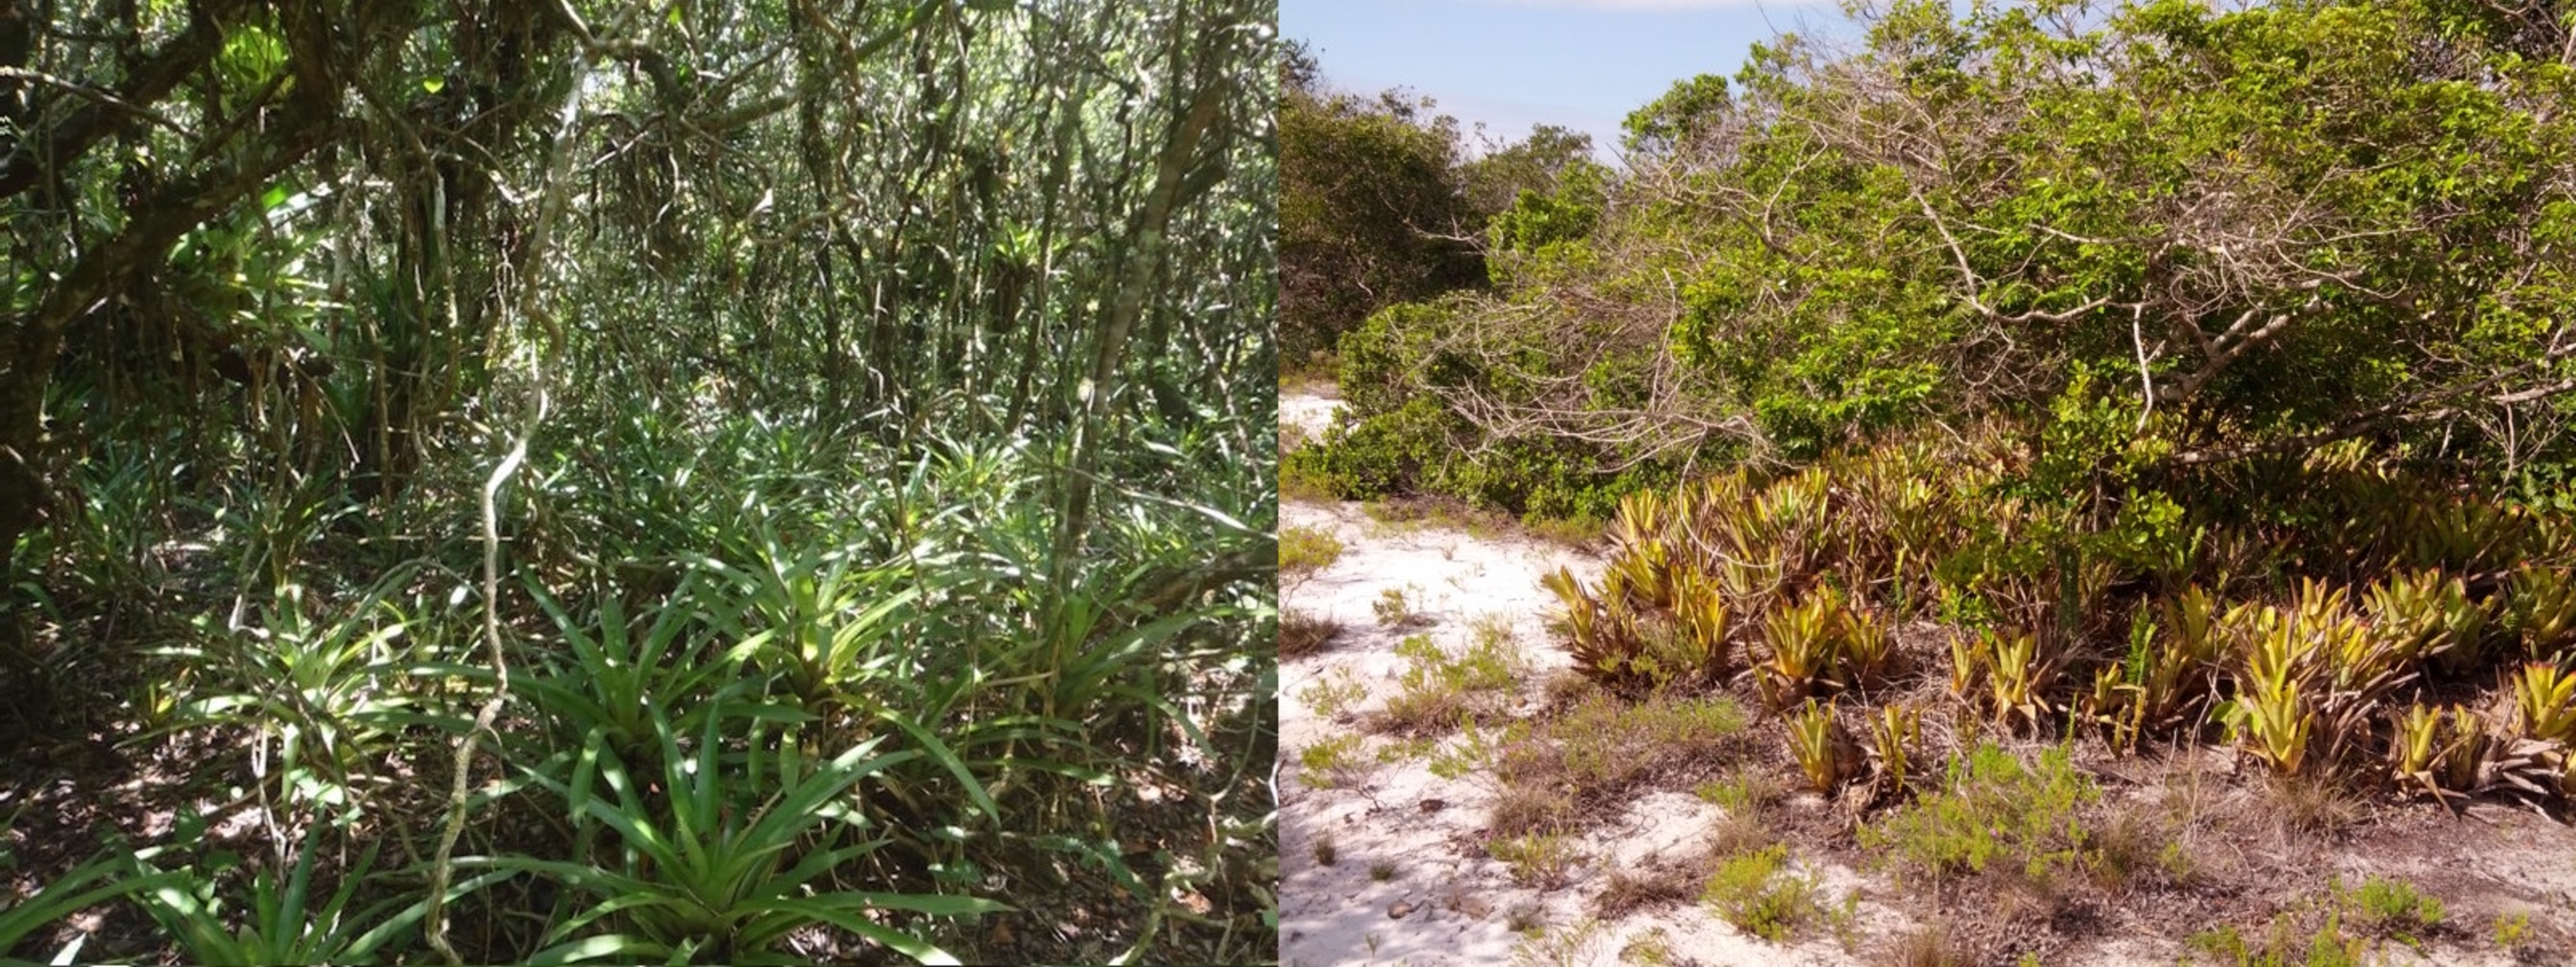
\includegraphics[width=5.5in]{figures/restinga2.pdf}
\caption[Photos of \emph{restinga} vegetation in Brazil]{Photos of \emph{restinga} vegetation in Brazil. \emph{Restingas} are dry, sandy habitats that occur in coastal sites within the Atlantic Rainforest in Brazil. On the left is a forested or ``closed'' restinga which was the location for Chapters 3 and 4. On the right is a more exposed or ``open'' restinga, the site of Chapter 2}
\label{fig:phylo_niche_overlap}
\end{figure}


In this thesis, I take the approach outlined above and apply it to the
tractable model system of bromeliad food webs. I use a combination of
observations and experiments to examine how deterministic and stochastic
processes affect the structure and functioning of these communities. In
each chapter I compare observations against specific null models, to
estimate which processes might be at work. Then, using manipulative
experiments, I test mechanisms suggested by the null models. I examine
two sources of ecological selection: the environment (abiotic) or other
organisms (biotic). Differences in the abiotic environment select for
the presence of different species; this is called habitat filtering.
Habitat filtering has many meanings \citep{Southwood1977, Kraft2015} but
in general refers to a conceptually simple process: among those subset
of species which arrive in a given patch, those who persist must be able
to tolerate both the abiotic and biotic conditions of that patch.

In Chapter 2, I consider the question of which types of organism
(bacteria, zooplankton or macroinvertebrates) show the strongest degree
of habitat filtering. Here, bromeliads offer a rare opportunity to
compare the community structure of these three organisms types -
differing in body size by many orders of magnitude- over the exact same
habitat gradient. In Chapter 3, I first identify the frequent
co-occurrence of predators with one another in bromeliads and overlap in
diets. This suggests the potential for strong predator-predator
interactions, which theoretically can have both antagonistic and
synergistic effects on prey. I use this as an opportunity to determine
how the phylogenetic diversity of predators affects their impact on prey
and ecosystem functions. In Chapter 4, I analyze the differences between
two congeneric species which have very different responses to habitat
size. In this chapter, I also demonstrate that invertebrate species that
live in bromeliads have a strikingly different response to bromeliad
size.

%%% Local Variables:
%%% TeX-master: "thesis"
%%% TeX-PDF-mode: t
%%% End:
